\section*{Kit content}

Each group receives one \textit{LELEC2102-3 kit} as shown in Fig.~\ref{fig:kit-content}.

\begin{figure}[h!]
    \centering
    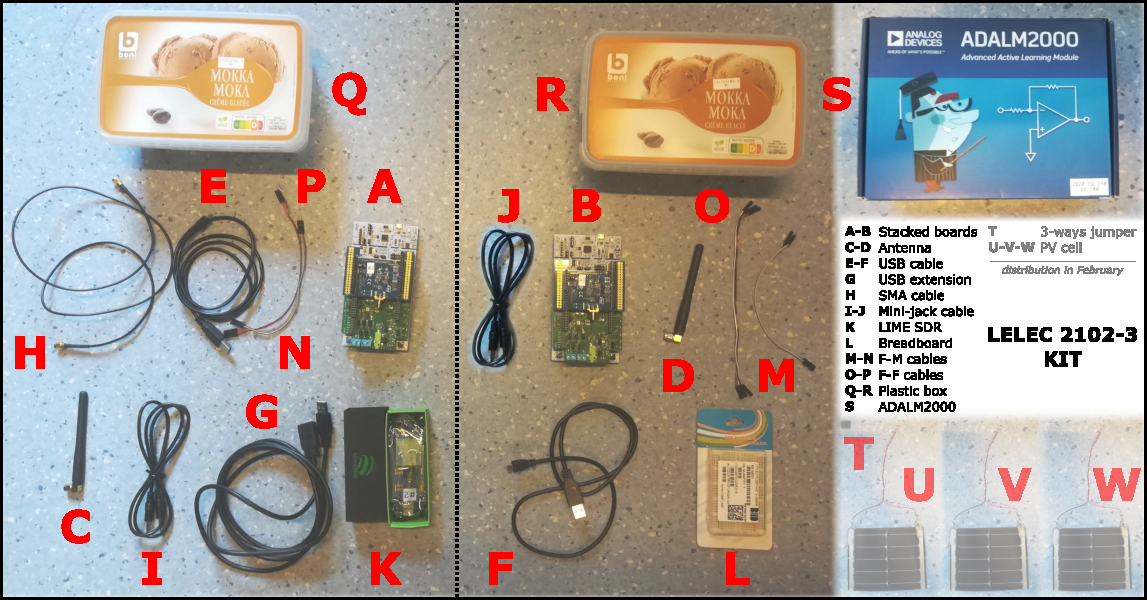
\includegraphics[width=1\textwidth]{figs/fig-contents.pdf}
    \caption{Kit content.}
    \label{fig:kit-content}
\end{figure}

Here is a detailed list of the hardware included in your kit:

\begin{itemize}
    \item 2$\times$ stacked boards (including \texttt{STM32L4A6 NUCLEO-144} MCU board, \texttt{Sub-1GHz 868MHz RF NUCLEO} radio board, \texttt{sensing and power-management} board);
    \item 2$\times$ antenna;
    \item 2$\times$ USB cable;
    \item 1$\times$ USB extension;
    \item 1$\times$ SMA cable;
    \item 2$\times$ mini-jack cable;
    \item 1$\times$ \texttt{LIME SDR};
    \item 1$\times$ breadboard;
    \item 2$\times$ female-male cables;
    \item 2$\times$ female-female cables;
    \item 1$\times$ \texttt{ADALM2000};
    \item \textcolor{gray}{2$\times$ male-male cable;}
    \item 3$\times$ PV cell with connectors \textit{(distribution in February)};
    \item 1$\times$ 3-ways jumper \textit{(distribution in February)}.

\end{itemize}

% \begin{bclogo}[couleur = gray!20, arrondi = 0.2, logo=\bcinfo]{Going below 3V3}
% Asym packs
% \end{bclogo}

Regarding the \texttt{ADALM2000}, please check that your box is similar to Fig.~\ref{fig:adalm}. More informations on the \texttt{ADALM2000} can be found on the \href{https://www.analog.com/en/design-center/evaluation-hardware-and-software/evaluation-boards-kits/ADALM2000.html#eb-overview}{website} of Analog Devices (click \href{https://wiki.analog.com/university/tools/m2k/users}{here} for a quick-start tutorial).

\begin{figure}[h!]
    \centering
    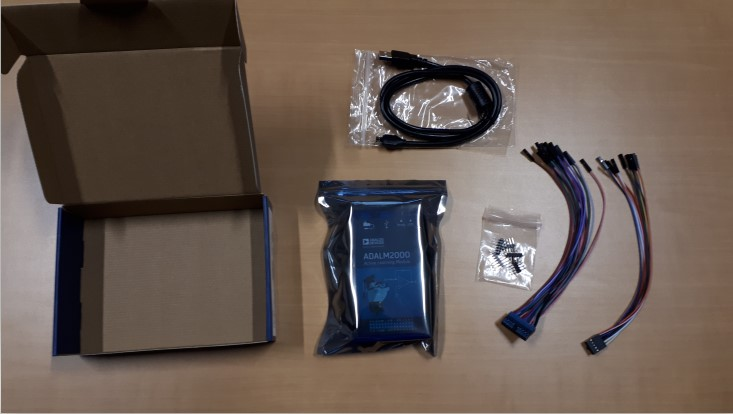
\includegraphics[width=1\textwidth]{figs/adalm.png}
    \caption{\texttt{ADALM2000} content.}
    \label{fig:adalm}
\end{figure}
